
%% -*-LaTeX-*- %%%%%%%%%%%%%%%%%%%%%%%%%%%%%%%%%%%%%%%%%%%%%%%%%%%%%%%
%%
%%%%%%%%%%%%%%%%%%%%%%%%%%%%%%%%%%%%%%%%%%%%%%%%%%%%%%%%%%%%%%%%%%%%%%

\documentclass{ict-doc}
\newcommand{\docproject}{E-Learning – VELS}
\newcommand{\doctitle}{E-Learning -- VELS}
\newcommand{\docsubtitle}{Usermanual}
\newcommand{\docauthors}{Martin Mosbeck, Andreas Platschek, Gilbert Markum, LingYin Huang}
\newcommand{\docreviewers}{Axel Jantsch}
\newcommand{\docversion}{0.9}
\newcommand{\docdate}{\today}
\newcommand{\doccopyrighta}{TU Wien,}
\newcommand{\doccopyrightb}{Institute of Computer Technology}

% Setup of the hyperref package

\hypersetup{, 
    colorlinks=false,
    bookmarks=true}

\usepackage{listings}
\usepackage{moreverb}
\usepackage{pdflscape}
\usepackage{todonotes}
\usepackage{longtable}
%\usepackage[T1]{fontenc} 
% The document, please keep the structure defined here

\begin{document}

\listoftodos

% Fill in the name of your docu-file.l


\begin{table}[h]
\begin{tabular*}{14.7cm}{|p{1,2cm}|p{4,0cm}|p{2cm}|p{5,8cm}|}
\hline
Version & Autor & Date & Comment \\[2pt]
\hline
\hline
0.1 & Martin Mosbeck & 14.09.2015 & First shot at User Manual. \\[2pt]
\hline
0.2 & Martin Mosbeck & 28.05.2016 & Updates for public release. \\[2pt]
\hline
0.3 & Martin Mosbeck & 04.10.16 & Updates about configurability. \\[2pt]
\hline
0.4 & Martin Mosbeck \par Gilbert Markum & 04.10.16 & Added Xilinx ISE ISim Install Notes \\[2pt]
\hline
0.5 & Martin Mosbeck & 27.05.17 & Rework, incorporation of changes to config file and system, incorporation of the
specification \\[2pt]
\hline
0.6 & Gilbert Markum \par Martin Mosbeck & 17.07.17 & Added section ``Creating a new task for the VELS system'' \\[2pt]
\hline
0.7 & LingYin Huang & 31.07.17 & Updates Debian 9 (Stretch) system prerequisites and minor typo correction in section "System Setup" \\[2pt]
\hline
0.8 & Martin Mosbeck & 20.09.17 & Inserted documentation for multi-language feature \\[2pt]
\hline
0.9 & Martin Mosbeck & 02.01.18 & Corrected typos, adding additional information to make documentation easier to
understand, section on task queue modes  \\[2pt]
\hline
1.0 & Martin Mosbeck & 09.07.18 & Deleted information about deleted skipping mode \\[2pt]
\hline
1.1 & Martin Mosbeck & 09.07.18 & Added information about TaskErrorNoticd message type\\[2pt]
\hline
1.2 & Martin Mosbeck & 01.11.18 & Restructuring of Prerequisites and adding QuestaSim notes.\\[2pt]
\hline
\end{tabular*}
\end{table}


\pagenumbering{arabic} % document with arabic page numbers

\section{Manual Overview} \label{overview}

The following document aims to inform an operator on on how the autosub system works
and how to configure and run a course using the autosub system. This manual is written
primarily for using autosub with VELS (VHDL E-Learning System). Nevertheless the autosub
system and the described structures are designed to be usable for diverse E-Learning
purposes.

The first part of this manual (Section \ref{system_interaction}) outlines the
interaction and use cases for a user and an operator with the E-Learning system.

The second part of this manual describes VELS, which itself can roughly be divided
into 3 parts:
\begin{enumerate}
    \item The autosub submission system (see Section \ref{autosub_system})
    \item The configuration and status web interface VELS\_WEB (see Section
	      \ref{VELS_WEB})
    \item The tasks interface (see Section \ref{tasks_system})
\end{enumerate}

The third part of this manual depicts prequesites (see Section \ref{system_prerequisites})
and whicht steps have to be taken for system setup (see Section \ref{system_setup}).

The fourth part describes how to create new tasks for VELS (see Section \ref{create_new_task}).

The Appendix (Section \ref{appendix}) list Implementational details of VELS.

\section{System Interaction} \label{system_interaction}
The VELS system is an E-Learning system for students who are learning the \gls{vhdl}. The
interaction between students and the system is solely via E-Mail. Configuration of the
system is done with a configuration file (for configuration items that can not change dur-
ing runtime) and a web interface (for configuration items that can change dynamically).

The VELS E-Learning system has 2 distinctive user groups: course operators and students. 
To satisfy the use cases for each of the 2 user groups the following interfaces have
been defined:
\begin{itemize}
\item VELS E-Mail Interface
\item VELS Web Interface
\item VELS Direct Server Access
\end{itemize} 

The different use cases for students and operator and the responsible interface can be 
seen in Table \ref{tab:usestudent} and Table \ref{tab:useoperator}.

\begin{table}[h]
\centering
\begin{tabular}{||l | l||} 
    \hline
    Use Case & Responsible interface \\ [0.5ex] 
    \hline\hline
    register with the system & VELS E-Mail Interface
    \\
    \hline
    get status in course & VELS E-Mail Interface 
    \\
    \hline
    request/get a task & VELS E-Mail Interface 
    \\
    \hline
    submit a task solution & VELS E-Mail Interface
    \\
    \hline
    ask a question & VELS E-Mail Interface
    \\
    \hline
\end{tabular}
\caption{Use cases for students}
\label{tab:usestudent}
\end{table}


\begin{table}[h]
\centering
\begin{tabular}{||l | l||} 
    \hline
    Use Case & Responsible interface \\ [0.5ex] 
    \hline\hline
    configure a course & VELS Web Interface
    \\
    \hline
    configure a task queue & VELS Web Interface
    \\
    \hline
    modify task generation or testbench generation & VELS Direct Server Access
    \\
    \hline
    create a new task & VELS Direct Server Access
    \\
    \hline
    view the progress for students & VELS Web Interface
    \\
    \hline
    view task statistics & VELS Web Interface
    \\
    \hline
    read log files & VELS Direct Server Access 
    \\
    \hline
\end{tabular}
\caption{Use cases for course operators}
\label{tab:useoperator}
\end{table}

\newpage

\subsection{VELS E-Mail Interface}\label{emailinterface}
The VELS E-Mail Interface is the primary interface for students. Students are uniquely 
identified by their E-Mail address to interact with this interface. The student has to 
interact with a single, non-changing E-Mail address during the whole duration of a course. 
These E-Mail addresses have to be added to the system's whitelist by a course operator 
in order to enable them to be authorized for interaction. If a user that is not on the 
whitelist sends an E-Mail to the system, the system replies with a message to use the 
whitelisted address or contact a course operator.

The different actions a student can take are defined via E-Mail subject and address. The 
following cases when using a whitelisted E-Mail address and system reactions are implemented:
\begin{itemize}
\item \textit{Arbitrary Subject, user not registered:} Registration is initiated. Registration with the 
	system creates the appropriate data entries in the database for the student. If adding the new user was 
	successful, the user gets an welcome E-Mail with general information on how the system works.
\item \textit{Subject contains the word "Question":} The student has a question about the course, this 
	question is forwarded to all course operators. The student receives a confirmation that the 
    question has been passed on.
\item \textit{Subject contains the phrase "Question Task N" where N is the task number:} The student 
    has a question about a specific task of the course, this question is forwarded to all task operators 
	for task N. The student receives a confirmation that the question has been passed on.
\item \textit{Subject contains the phrase "Result Task N" where N is the task number:} The student wants 
    to hand in a solution, for Task N. Students are allowed to hand in solutions for all tasks that 
    have already been solved previously, as well as the one task that has not been solved yet -- they
    are not allowed to hand in solutions for tasks they did not receive the task description yet. The
    solution is tested on the server. If the task solution was appropriate the student will receive the
    next task (or a congratulations message, if no more examples are available). If the tests were not
    successful, the student receives an error message that gives a hint on what may be wrong (output of the
    simulation tool, expected output vs. actual output, etc.)
\item \textit{Subject contains the word "Status":} The student is send an E-Mail with the list of
    his completed tasks and his current task description.
\item \textit{\textit{default:}} The student is sent an E-Mail with the usage for this interface.
\end{itemize}

\newpage 

Depending on the chosen task queue mode additional keywords are accepted (for a closer description of different modes 
look at Section \ref{sub:task_queues}):

\textbf{With request mode:}
\begin{itemize}
\item \textit{Subject contains the word "Request Task N":} The student wants to request the task N. If the task can be 
	given to the student at this moment, the student will receive an E-Mail containing all informations on the task.
\end{itemize}

\textbf{With linear mode and skipping allowed:}
\begin{itemize}
\item \textit{Subject contains the word "Skip":} The student will be skipped to the task after his current task if 
	this task can be given to the student at this moment and will receive an E-Mail containing all informations on 
	the task.
\end{itemize}


\subsection{VELS Web Interface}\label{webinterface}

The VELS Web Interface is a configuration and status tool for the course operators.

Course operators can create a course. A course consists of a task queue which is a selection of the available tasks.
The following actions for course configuration  are implemented:
\begin{itemize}
\item Configuration of the task queue
\item Configure course registration deadline
\item Modify course registration E-Mail whitelist 
\item Modify archive directory
\item Set administrator E-Mail
\end{itemize}

Course operators can view the progress of each student and is presented with the following informations:
\begin{itemize}
\item Student name.
\item Task the student is working on and the tasks the student has completed.
\item Score which was accumulated by the student.
\item Number of submissions for each task the student has received.
\item List of attached files for each task the student has received.
\end{itemize}

Course operators can view statistical informations about their course:
\begin{itemize}
\item Number of wrong and right submissions for each task.
\item General statistical informations about the course (e.g number E-Mails received/sent).
\end{itemize}

The VELS Web Interface may also be used by the course operator to read the results at the end of the semester,
that is the points that have been scored by the individual students. In depth description on how to use the 
VELS\_WEB interface can be found in Section \ref{VELS_WEB} and Section \ref{system_setup}.


\subsection{VELS Direct Server Access}\label{directserveraccess}
The VELS Direct Server Access is used by course operators to  modify code for task
generation, description and testing of existing tasks, read log files or fix bugs of the VELS system. 
It also can be used to view every submission a student has done. 

\section{Autosub Submission System} \label{autosub_system}

The autosub submission system has the following responsibilities:
\begin{itemize}
    \item Fetch, process, send and archive student E-Mails.
    \item Store and manage tasks, users and submissions.
    \item Initiate generation of tasks and testing of submissions.
    \item Produce statistics.
\end{itemize}

In the following {\it Structured Analysis} will be used to specify the
system. If you are not familiar with this method, you can find details e.g. in
\cite{demarco, gooma, cooling}.

\begin{figure}[h!]
    \begin{center}
    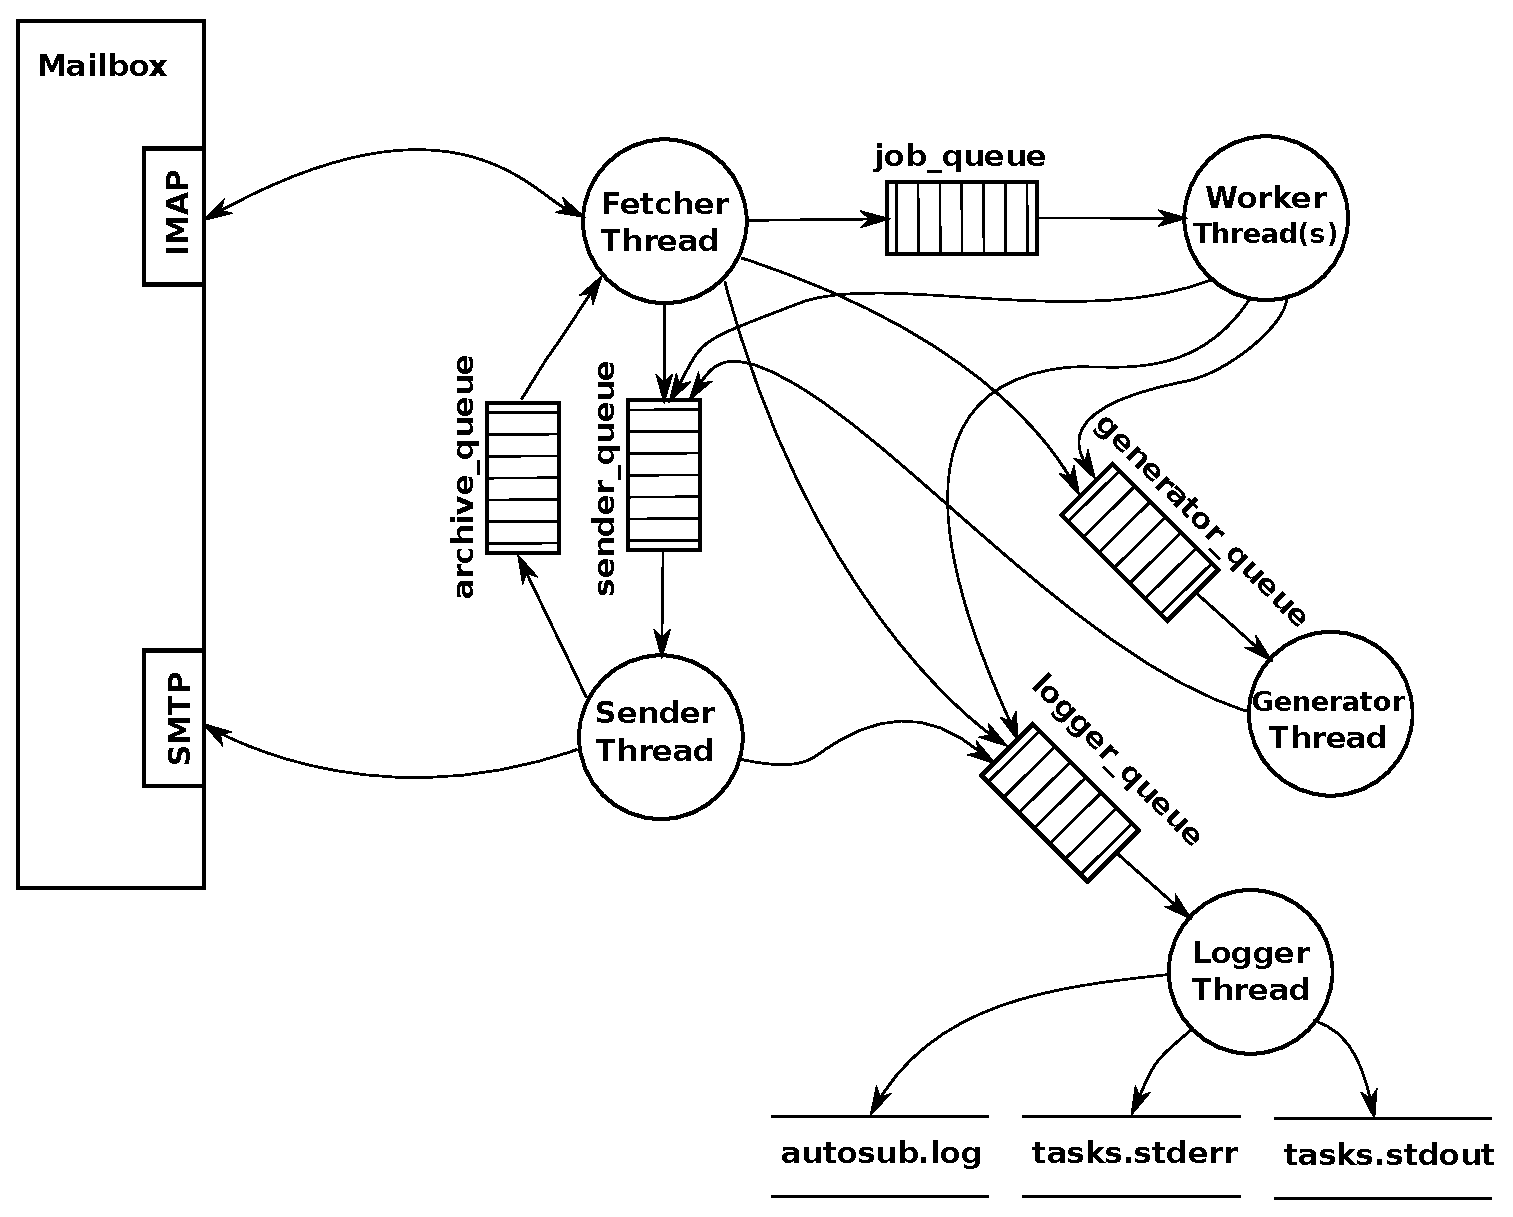
\includegraphics[width=11cm]{images/autosub_structure.eps}
    \caption{DFD0 -- High-Level Data-Flows in the Submission System.}
    \label{fig:dfd0}
    \end{center}
\end{figure}

The autosub submission system is a daemon implemented in Python3 that is 
composed of multiple threads communicating over queues. This multi-threading 
approach is especially important for the testing process. As the test of a single
task can take rather long and each student can hand in (correct and incorrect) 
solutions. Furthermore the goal is to assure, that there still is progress, even 
if a test is running. A view of the parts and data-flows of the autosub system can 
be seen in Figure \ref{fig:dfd0}. The individual entities are described in the next subsection,
the message queues in the Appendix Section \ref{app:queues}.

\subsection{Description of Entities} \label{autosub_entities}
\begin{description}
    \item [MB] \textbf{Mailbox} \\
    \begin{tabular}{|p{2cm}|p{11cm}|}
        \hline
        Description & Mailbox to interface with students. \\
        \hline
        Rate & Asynchronously by students, periodically with configurable interval by
		the E-Learning system. \\
        \hline

        Comment & The Mailbox is used to interface with the students.
        The Mailbox is accessed via \gls{imap} for reading new E-Mails and \gls{smtp} 
		to send E-Mails.

        After the action triggered by an received E-Mail has been processed, the E-Mail 
		is archived into a configurable folder on the \gls{imap} server.
        \\
        \hline
    \end{tabular}
    \item [1] \textbf{Fetcher thread} \\
    \begin{tabular}{|p{2cm}|p{11cm}|}
        \hline
        Description &  Fetch E-Mails from the Mailbox.\\
        \hline
        Rate & Periodically with configurable interval. \\
        \hline
        Comment & The Fetcher thread periodically checks the Mailbox for new E-Mails. 
		This thread initiates actions based on the user E-mail address and the subject.
		Further information concerning the E-Mail interface can be be seen in Section 
		\ref{emailinterface} 
        \\
        \hline
    \end{tabular}

	\item [2] \textbf{Generator thread} \\
    \begin{tabular}{|p{2cm}|p{11cm}|}
        \hline
        Description & Generate a (unique) example for a user. \\
        \hline
        Rate & Triggered by registration of a new user, and successful submission 
		of a task.  \\
        \hline
        Comment & The Generator thread initiates generation of unique tasks for students.
  		The Generator thread is blocking on the generator\_queue, until the generation 
		of a new example is requested. As soon as the example was generated, a request 
		to send it out is put into the sender\_queue.
        \\
        \hline
    \end{tabular}
   
	\item [3] \textbf{Worker thread(s)} \\
    \begin{tabular}{|p{2cm}|p{11cm}|}
        \hline
        Description & Test the task submissions of students. \\
        \hline
        Rate & Asynchronously triggered upon arrival of a new task submission 
		by a student. \\
        \hline
        Comment & The Worker threads are the ones which do the initiate testing 
		submissions by a student. If the Fetcher thread receives an E-Mail with a result 
		submission, a new message is added to the job\_queue. The worker threads are 
		using a blocking read on the job\_queue to wait for work, as soon as the new 
		message is added by the Fetcher thread one of the workers will read it and 
		start the tests for the users submission.
        \\
        \hline
    \end{tabular}

    
	\item [4] \textbf{Logger thread}\label{sec:logger} \\
    \begin{tabular}{|p{2cm}|p{11cm}|}
        \hline
        Description & Format log messages and store them in the log file. \\
        \hline
        Rate & Triggered by all other threads. \\
        \hline
		Comment & In order to enforce a common logging format, and allow the setting 
		of a common log-level, all threads just put their log-messages into the 
		logger\_queue. The Logger thread decides (depending on the log-level and configured 
		log-threshhold) whether or not the message shall be logged or not. If so, the message
		is formatted and written to the log file. The log-level threshold can be configured in the
		config file.

		The following log-levels are implemented (from lowest to highest):
        \begin{description}
		\item [DEBUG:] Print all kind of information that might be helpful to debug
			problems. This includes, what user sent which e-mail, what action
			was taken, what was the result of that action.
		\item [INFO:] Information that might be of interest, even if not in debugging
			mode.
		\item [WARNING:] A problem occurred, but it did not lead to a long-term problem
			(e.g. could not connect to the mailserver, but after retrying it worked).
		\item [ERROR:] A problem that lead to a long-term malfunction of the submission
			system occurred, the system will not be able to recover from this problem.
		\end{description}
        \\
        \hline
    \end{tabular}

	\item [5] \textbf{Sender thread} \\
    \begin{tabular}{|p{2cm}|p{11cm}|}
        \hline
        Description & Sends E-Mails to the students \\
        \hline
        Rate & Triggered by Fetcher, Worker or Generator thread. \\
		\hline
		Comment & If a message has to be returned to the student, the thread that 
		wants to send the message just puts the necessary information into the 
		sender\_queue. The sender thread then takes that information, formats an 
		e-mail and sends it out using \gls{smtp}.

        The unique message-id is passed from the fetcher (possibly via other 
		threads) to the sender thread. If the sender thread has sent out the 
		answering E-Mails, the E-Mail with the given message-id is moved into an 
		archive folder on the mail server.
        \\
        \hline
    \end{tabular}

	\newpage 

	\item [6] \textbf{Dailystats thread} \\
    \begin{tabular}{|p{2cm}|p{11cm}|}
        \hline
        Description & Creates statistical information. \\
        \hline
        Rate & Activated every 12 hours. \\
		\hline
		Comment & The dailystats thread is used to get a timeline of some very basic statistics.
		Currently the number users, sent e-mails, received e-mails and received questions
		over time are evaluated and plotted into a graph. The graphs are stored and 
		can e.g. be viewed in the Statistics tab of the web interface.
        \\
        \hline

    \end{tabular}
\end{description}

\subsection{Datastores}
For storing data two databases are used. The name and location of those databases 
can be configured through the configuration file, in the following we will refer to 
them with the default name that is used, if no other name is provided in the 
configuration file:
\begin{description}
\item [semester.db: ] The {\tt semester.db} database is used to store all data that is
    specific to one semester. This includes, users, parameterization of tasks assigned
    for users, statistics, etc. The {\tt semester.db} default location is in
	{\tt "autosub/src"}.
\item [course.db: ] The {\tt course.db} database consists of configuration data that will
    very likely be reused in multiple semesters. This separation makes it very easy
    to start a new semester: just backup {\tt semester.db} to some safe location and
    remove it in the original location (a new empty one will be made automatically upon 
    starting the autosub daemon). Then use the VELS web interface to perform the small 
    modifcations(year/semester,deadlines, etc.) needed in {\tt course.db}. The
    {\tt course.db} default location is in {\tt "autosub/src"}.
\end{description}
Specifics about the tables of these databases can be found in the Appendix Section
\ref{app:semester.db} and \ref{app:course.db}.

In addition there is one important directory that is used by autosub to store data in,
the directory: {\tt autosub/src/users}. In this directory a unique directory for every
user is created, and this directory the description of each individual received task 
and submissions for the individual tasks are stored. Every directory has the form 
{\tt "autosub/src/users/<user\_id>/Task<nr>/"}. Submissions are stored in separate 
folders which are named {\tt "Submission<nr>\_<date>\_<time>/"}. Task description files 
are stored in the folder named {\tt "desc/"}.

\subsection{Config File}
The autosub system uses a config file (.cfg) which is passed to the daemon to configure the
individual threads and overall system. The file is read when starting the daemon. If no
.cfg file is specified, the used file is default.cfg located in {\tt "autosub/src/"}. 
Information about the config file can be found in the Appendix Section \ref{app:config}
and an example config filein in Section \ref{sub:exampleconfig}.

\subsection{Logging and error detection} \label{logerror}

The autosub system is implemented as a daemon process. As such it does not
directly print any information to the {\tt stdout} (i.e. the screen), instead
all messages for the administrator are stored in log files. All log and error files
are stored in a configurable directory (default {\tt "autosub/src"}).

\begin{description}
\item [autosub.log] This is the main log file that is used by the actual autosub
daemon software to log everything. The format in this log file is as follows:

\begin{verbatim}
<date> <time> [<logger name>] <loglevel> <logmessage>
\end{verbatim}

Here is a small section of {\tt autosub.log} taken from startup -- first the daemon checks
whether a directory {\tt users} used to store the users submissions is existing, then
it checks if necessary tables in the database exist. After those checks have been
done further threads (described in Section \ref{autosub_entities}) are started, and
announce themselves.

{\scriptsize
\begin{verbatim}
2015-09-17 22:23:40,629 [autosub.py  ] WARNING: Directory already exists: users
2015-09-17 22:23:40,630 [autosub.py  ] DEBUG: table SpecialMessages does not exist
2015-09-17 22:23:43,679 [autosub.py  ] DEBUG: table TaskConfiguration does not exist
2015-09-17 22:23:43,955 [autosub.py  ] DEBUG: table GeneralConfig does not exist
2015-09-17 22:23:45,878 [sender      ] INFO: Starting Mail Sender Thread!
2015-09-17 22:23:45,884 [fetcher     ] INFO: Starting Mail Fetcher Thread!
2015-09-17 22:23:45,884 [fetcher     ] DEBUG: Imapserver: 'mail.intern.tuwien.ac.at'
2015-09-17 22:23:45,884 [generator   ] INFO: Task Generator thread started
2015-09-17 22:23:45,890 [activator   ] INFO: Starting activator
2015-09-17 22:23:45,890 [Main        ] INFO: Used config-file: testzid.cfg
2015-09-17 22:23:45,891 [Worker1     ] INFO: Starting Worker1
2015-09-17 22:23:45,892 [Main        ] INFO: All threads started successfully
2015-09-17 22:23:45,892 [Worker1     ] INFO: Worker1: waiting for a new job.
2015-09-17 22:23:45,893 [Worker2     ] INFO: Starting Worker2
\end{verbatim}
}

As you can see from theses examples, a lot of information is available, with
exact timestamps and a way to know which thread the message is coming from.
In addition the debug level gives a sense of how important (or even critical)
the message is. The log-level threshhold can be configured using the config file.

\end{description}

Autosub tries to give information on severe problems on all available channels. An example would be,
if no task is configured, the email sent to the student will contain the message that
something went wrong as well -- although the error can be seen in the {\tt autosub.log}
file as well.


\section{The web inteface VELS\_WEB} \label{VELS_WEB}

The configuration and status web interface VELS\_WEB was designed as an easy interface
for a course operator to view and change course parameters and monitor the course progress.
It is implemented with web2py and can be run as a daemon accessing the datastores of the
autosub submission system. This web interface was only 
designed for internal operator use! Therefore it should only be reachable via 
the internal networks using a web browser.

The menu items of the VELS\_WEB are the following:
\begin{description}
\item [Start:] The start page.
\item [Users:] View of the registered students, allows to change or a student via the
    "Edit" button, delete a student via the "Delete" button  and show the progress of
    a student in the course via the "View" button. The table is sortable by column by
    clicking on the head of the column.
\item [Tasks:] The task configuration, will be discussed in Section \ref{sub:configTasks}.
\item [Whitelist:] Change whitelisting for students, will be discussed in Section
    \ref{sub:whitelisting}.
\item [General Config:] Change dynamic configuration items of VELS, will be discussed in
    Section \ref{sub:generalconfig}.
\item [Statistics:] View statistics about sent and received emails and task success of
    the students.
\item [User Tasks:] View mappings from students to individual tasks.
\end{description}

Usage of the VELS\_WEB interface will be discussed with system setup in Section \ref{system_setup}.

\section{The Tasks System} \label{tasks_system}

\subsection{Minimal and optional task structure}

Every task is located in an individual folder in the tasks directory (configurable via 
the autosub config file). Certain structures with minimum behavior are needed in order 
to use the task with the autosub system. In detail instructions how to create a taks can 
be found in Section \ref{create_new_task}.

\begin{tabular}{|p{3cm}|p{10cm}|}
\hline

Minimal & \begin{itemize}
    \item {\bf Generator executable:} Generates random task parameters for the task, 
		creates entity and behavioral vhdl files and description pdf file for the student. Copies
		these files to the user taskpath ({\tt "autosub/src/users/<user\_id>/Task<nr>/"}). Declares
		which files shall be attached to the task description E-Mail and the task parametes and 
		adds them to the autosub system using the tool {\tt "autosub/src/tools/add\_to\_usertasks.py"}.
    \item {\bf Tester executable:} Given the individual task parameters, tries to test
		the student's solution located in {\tt "autosub/src/users/<user\_id>/Task<nr>/"}. 
		Generates an individual testbench for the student's solution. Tests 
        the solution and creates feedback textfile {\tt "error\_msg"}, error attachments in the directory
		{\tt "error\_attachments"} and tells the autosub system the test result via returncode
    \item {\bf description.txt:} Contains a textual task description. The text in description.txt 
    	is sent to the user as the body of the E-Mail that contains a new task description.
	\end{itemize} 
\\
\hline
\end{tabular}

\newpage

Certain optional structures have proven to be useful.

\begin{tabular}{|p{3cm}|p{10cm}|}
\hline

Optional & \begin{itemize}
    \item {\bf Directory scripts:} Scripts that are called from the executables in order to aid the 
        generation or test process
    \item {\bf Directory templates:} Files that are filled with parameters and can be used to generate entity 
        declarations, testbenches, description files.
    \item {\bf Directory static:} Files that are static for the task, therefore the same for every student.
    \item {\bf Directory exam:} Files that are needed for the VELS exam mode.
\end{itemize} 
\\
\hline
\end{tabular} 

An usual sequence for the task generation in VELS is:
\begin{enumerate}
    \item The generator executable is called by the autosub Generator thread.
    \item The generator executable calls a task generation script
        {\tt "scripts/generateTask.py"}.
    \item The task generation script generates random task parameters and returns
        them, fills a LaTeX description template and vhdl templates and stores
        the results in the directory {\tt "tmp/"}.
    \item The generator executable generates the task description pdf file from the
        filled template and copies it, all filled vhdl files and static vhdl files
        to the users task description path {\tt "autosub/src/users/<user\_id>/Task<task\_nr>/desc/"}.
    \item The generator executable calls {\tt "autosub/src/tools/add\_to\_usertasks.py"} 
		with the task parameters and path to files that belong to the individual student task. 
		This tool saves these informations per user in the semester database for creation of the
		student task E-mail.
\end{enumerate}

An usual sequence for submission testing in VELS is:
\begin{enumerate}
\item The tester executable is called by a autosub Worker thread.
\item The tester executable calls a testbench generation script
    {\tt "scripts/generateTestBench.py"}.
\item The tesbench generation script creates a testbench with test vectors and returns it.
\item The tester executable stores the testbench in the user task directory 
	{\tt "autosub/src/users/<user\_id>/Task<task\_nr>"} and copies needed files from the user task
    description path {\tt "autosub/src/users/<user\_id>/Task<task\_nr>/desc"} to the user task directory 
	{\tt"autosub/src/users/<user\_id>/Task<task\_nr>"}.
\item The tester executable checks if the needed submission files are present in the
	user task directory. These files are stored from E-Mail attachments by the Fetcher thread. If they are
	not present an error is written to a {\tt error\_msg} file and the process returns failure. This initiates
	the sending of an E-Mail to the student.
\item The tester executable analyzes files generated by the task system, if errors
    occur the process stops stops and returns a task error. This initiates the sending of an E-Mail to the student 
	and system administrators.
\item The tester executable analyzes the student submission files, if errors occur they
    are written to a {\tt error\_msg} file and the process stops and returns failure. This initiates
	the sending of an E-Mail to the student.
\item The tester elaborates and runs the testbench, if the tests fail meaningful messages
    are written to a {\tt error\_msg} file, the process stops and returns failure. If the test was successfull the 
	{\tt error\_msg} file remains emty and the tester returns success. Both cases initiate
	the sending of an E-Mail to the student.

\end{enumerate}

\subsection{Tasks error detection and logging} \label{tasklog}
The autosub daemon calls generator and tester scripts for the individual tasks. The logging 
of these scripts is done by piping the output of called generator and tester scripts into 
seperate log files. All output to stdout is piped into the logfile {\tt tasks.stdout}, allo 
error output to stderr is piped into the logfile {\tt tasks.stderr}. The location of these
files (default {\tt "autosub/src"}) can be configured using the log file. Messages to the 
files are logged in the format:
\begin{verbatim}
--------------------------------------------------------------------
<date> <time> [Task<task_nr>(<worker_nr)] <ERROR/INFO>:
--------------------------------------------------------------------
<logmessage>
\end{verbatim}

\newpage 

An example for the tester of a submission from the gates task to {\tt tasks.stdout} is:
{\scriptsize
\begin{verbatim}

--------------------------------------------------------------------------------
2017-05-09 15:07:16,124 [Tester1(10) ]INFO:
--------------------------------------------------------------------------------
Parsing VHDL file "gates.vhdl" into library work
Parsing VHDL file "gates_tb_10_Task1.vhdl" into library work
Parsing VHDL file "IEEE_1164_Gates_pkg.vhdl" into library work
Parsing VHDL file "IEEE_1164_Gates.vhdl" into library work
Parsing VHDL file "IEEE_1164_Gates_beh.vhdl" into library work
Parsing VHDL file "gates_beh.vhdl" into library work
Task 1 analyze success for user 10!
Task 1 not using the provided gate entities for user 10!
\end{verbatim}
}

\section{VELS Pre-Requisites} \label{system_prerequisites}

In the following, the installation of pre-requisites for autosub is documented for 
the two current debian versions. Wheezy is currently the old-stable which was used 
for development of autosub, and jessie is the current stable which has been used to 
test autosub as well.

\subsection{Debian 7 (Wheezy)}

The probably easiest step is to install standard debian packages:

\begin{verbatim}
apt-get install python3 python3-mock python3-pip python3-nose zip flip git
apt-get install gnat-4.6-base libgnat-4.6 texlive-latex-extra pgf graphviz
apt-get build-dep python-matplotlib
\end{verbatim}

Unfortunately there is a small bug in one of the latex packages that we use,
therefore you need to apply a patch to that package:

\begin{verbatim}
cd /usr/share/texlive/texmf-dist/tex/generic/pst-circ
patch < /path/to/autosub/doc/patch/pst-circ.tex.patch
\end{verbatim}

In case the pdfs you get are not beautiful as you are used to, it might have
happended that an update was applied over that patch and you need to re-apply it (sorry for that little mess).


Next we need to upgrade easy\_install for python3 to a newer version -- this
is the pre-requisite for the installation of the matplotlib for python3.

\begin{verbatim}
easy_install3 -U distribute
\end{verbatim}

And finally we may now install some libraries that are not (yet) available in
the debian package system via using pip:

\begin{verbatim}
pip-3.2 install graphviz
pip-3.2 install bitstring
pip-3.2 install matplotlib
\end{verbatim}

Last, we install a vhdl simulator. If you want to use ghdl you may download
the debian package from sourceforge \footnote{http://sourceforge.net/projects/ghdl-updates/files/Builds/ghdl-0.31/Debian/} and install it using dpkg:

\begin{verbatim}
dpkg -i Downloads/ghdl_0.31-2wheezy1_amd64.deb
\end{verbatim}

All the dependencies of that package have already been resolved by the above
list of packages installed with apt.

To use the Simulator of Xilinx's ISE: ISim, see Section \ref{ISE-install}

At this point you may run the test-suite, as explained in Section \ref{sub:testingvels}.
If those tests run through without complications, everything you need to run the VELS
E-Learning system has been installed successfully.

\subsection{Debian 8 (Jessie)}

For jessie everything is even easier as more libraries are available for python3 in the
apt package pool now:

\begin{verbatim}
apt-get install python3 python3-mock zip flip graphviz python3-pip
apt-get install python3-matplotlib python3-nose gnat-4.9-base libgnat-4.9
apt-get install zlib1g-dev texlive-latex-extra pgf git
\end{verbatim}

Unfortunately there is a small bug in one of the latex packages that we use,
therefore you need to apply a patch to that package:

\begin{verbatim}
cd /usr/share/texlive/texmf-dist/tex/generic/pst-circ
patch < /path/to/autosub/doc/patch/pst-circ.tex.patch
\end{verbatim}

In case the pdfs you get are not beautiful as you are used to, it might have
happended that an update was applied over that patch and you need to re-apply it (sorry for that little mess).

So now, only two more packages that need to be installed using pip:

\begin{verbatim}
pip3 install bitstring
pip3 install graphviz
\end{verbatim}

Last, we install a vhdl simulator. If you want to use ghdl there you can use the version from \footnote{http://sourceforge.net/projects/ghdl-updates/files/Builds/ghdl-0.33/debian/} as there are no .deb packages for jessie of the older ghdl version (and vice-versa).

\begin{verbatim}
dpkg -i ghdl_0.33-1jessie1_amd64.deb
\end{verbatim}

To use the Simulator of Xilinx's ISE: ISim, see Section \ref{ISE-install}

At this point you may run the test-suite, as explained in Section \ref{sub:testingvels}.
If those tests run through without complications, everything you need to run the VELS
E-Learning system has been installed successfully.

\subsection{Debian 9 (Stretch)}

For stretch the standard debian packages are available for installation by:

\begin{verbatim}
apt-get install python3 python3-mock zip flip graphviz python3-pip
apt-get install python3-matplotlib python3-nose gnat-6 libgnat-6
apt-get install zlib1g-dev texlive-latex-extra pgf git python3-pygt5
\end{verbatim}

Unfortunately there is a small bug in one of the latex packages that we use,
therefore you need to apply a patch to that package:

\begin{verbatim}
cd /usr/share/texlive/texmf-dist/tex/generic/pst-circ
patch < /path/to/autosub/doc/patch/pst-circ.tex.patch
\end{verbatim}

In case the pdfs you get are not beautiful as you are used to, it might have
happended that an update was applied over that patch and you need to re-apply it (sorry for that little mess).

So now, only two more packages that need to be installed using pip:

\begin{verbatim}
pip3 install bitstring
pip3 install graphviz
\end{verbatim}

Last, we install a vhdl simulator. The simulator of Xilinx's ISE installation is recommended since there is no dedicated
version of vhdl for Debian stretch. 
If you still want to use ghdl you can try the version described in Debian 8 (Jessie).

\begin{verbatim}
dpkg -i ghdl_0.33-1jessie1_amd64.deb
\end{verbatim}

To use the Simulator of Xilinx's ISE: ISim, see Section \ref{ISE-install}

At this point you may run the test-suite, as explained in Section \ref{sub:testingvels}.
If those tests run through without complications, everything you need to run the VELS
E-Learning system has been installed successfully.

\subsection{Instalation Notes for Xilinx ISE 14.7}\label{ISE-install}

An additional option, to using the open-source software ghdl as the VHDL Simulation tool for VELS, is to use the Simulator of Xilinx's ISE: ISim. The ISE (``Full Installer for Linux'') can be downloaded from Xilinx's official download page. It requires registration and licensing agreement, but there is no charge.

For installing ISE to the default location /opt/Xilinx/ where the VELS system expects it to be, you need permission to write to this location. So we will use the user root to call the graphical installer. To do so we need to allow root to use the users X server. As a user run:

\begin{verbatim}
$ xhost +
\end{verbatim}

to allow root (or anyone) to connect to your users X server temporarily. Now as root start the graphical installer, located at the top of the extracted download, with

\begin{verbatim}
# ./xsetup
\end{verbatim}

In case that you are using the KDE desktop environment, you have to remove the \verb!QT_PLUGIN_PATH! environment variable before starting the graphical installer:

\begin{verbatim}
# unset QT_PLUGIN_PATH
\end{verbatim}

If you are running the VELS system on a machine without a graphical user interface, the best way we found to get Xilinx's ISE onto a remote debian server was to copy the entire installation directory after it has been installed on a non-headless machine.

\section{Setting up the VELS system} \label{system_setup}

\subsection{VELS server setup} \label{sub:serversetup}

The first thing to do when you want to install the autosub submission system and the VELS
web interface is to clone the git repository:

\begin{verbatim}
git clone https://github.com/autosub-team/autosub.git
\end{verbatim}

\subsection{Configuration File Creation} \label{sub:exampleconfig}
The autosub config file is used to configure the connection to the mail server and set
configuration parameters for the system. In order to run the autosub daemon a config file
has to be created. The config file fields each belong to one of the groups embraced 
in [...]. An example config file can be seen below, the full list of fields and their
meaning is described in Appendix 
Section \ref{app:config}

\begin{lstlisting}[frame=single,captionpos=b,caption=example.cfg, belowcaptionskip=4pt]]
[imapserver]
servername: imap.gmail.com
serverport: 993
security: ssl
username: submission@gmail.com
password: mysupersecurepassword
email: submission@gmail.com

[smtpserver]
servername: smtp.gmail.com
serverport: 587
security: starttls
username: submission@gmail.com
password: mysupersecurepassword
email: submission@gmail.com

[system]
num_workers: 20
queue_size: 200
poll_period: 5
log_dir: /home/martin/autosub/src
log_threshhold: INFO

[course]
tasks_dir: /home/martin/autosub/tasks/implementation/VHDL
course_name: My Cool Course
mode: normal
allow_skipping: no
auto_advance: no
\end{lstlisting}

\subsection{Starting the Daemon}

Autosub is implemented as a daemon process, that means all messages provided are written
to files (see Section \ref{logerror} and \ref{tasklog} for details on those files) -- 
nothing is written to the console. The daemon is started using a shell-script located
in {\tt autosub/src/}:

\begin{verbatim}
./autosub.sh start
\end{verbatim}

This starts the daemon using the default configuration file named {\tt default.cfg}. If you
wan to use your own configuration file, you have to pass the files name to the scrip when
starting the daemon:

\begin{verbatim}
./autosub.sh start myconfig.cfg
\end{verbatim}

To stop the daemon just run the command:

\begin{verbatim}
./autosub.sh stop
\end{verbatim}

\subsection{Setting up the VELS\_WEB Configuration Interface}
To use the VELS\_WEB Configuration Interface it has first to be installed and
configured using these steps:

Change to the VELS\_WEB directory.

\begin{verbatim}
python3 installer.py <pathtoautosub> <pathtoconfigfile>
\end{verbatim}

Use the same configfile you used for starting the autosub daemon! This step will
also download web2py to the user's home folder and set needed symbolic links to 
connect VELS\_WEB to the autosub system.

If you change parameters in the category $[$system$]$ in your autosub config file or need to switch to 
another config file run the installer with the reinstall flag:

\begin{verbatim}
python3 installer.py --reinstall <pathtoautosub> <pathtoconfigfile>
\end{verbatim}

To use https you have to use a SSL key. The system expects the keyfiles
(server.crt , server.csr , server.key) to be in the web2py directory. To
generate keys and place them run the following (this can be skipped if you 
already have keyfiles you can use!):

\begin{verbatim}
./genkeys.sh    
\end{verbatim}

To start the VELS\_WEB daemon at port <port> and with web2py admin password 
<password> (this can be set by you!) run:
\begin{verbatim}
./daemon.sh start <port> <password> 
\end{verbatim}

After this step the VELS\_WEB interface will be reachable via your browser at
address:
\begin{verbatim}
https://<server_ip>:<port>/VELS_WEB
\end{verbatim}

To stop the daemon just run the command:

\begin{verbatim}
./daemon.sh stop
\end{verbatim}

\subsection{General Configuration}\label{sub:generalconfig}
Configuration items that can be changed dynamically are changeable in VELS\_WEB ->
General Config. These configurable items are:
\begin{itemize}
\item {\bf Registration Deadline:} Users who are try to register after this deadline will
    get an error e-mail.
\item {\bf Archive Directory:} Directory in which processed e-mails are moved, this
    directory has to be present on the IMAP server!
\item {\bf Administration E-Mail:} E-Mail addresses which get question and system error E-Mails.

\end{itemize}

\subsection{Whitelisting} \label{sub:whitelisting}
Students that participate in the course have to be whitelisted in the VELS system. If the student
tries to write an E-Mail to the system from an E-Mail address that is not on the Whitelist, an E-Mail
with an error message is sent to him.

Whitelisting can be done in VELS\_WEB under the tab {\it Whitelist}. E-Mail addresses can be added
one at a time or multiple at a time (mass subscription). Removal of a single E-Mail address
can also be done in the VELS\_WEB. Names which will be used when users register can also be 
specified. This is usefull, because many users don't send E-Mails with their name configured
in the "From" header.

\subsection{Configuring the Tasks} \label{sub:configTasks}
Existing tasks can be assembled into a task queue. This configuration is done in VELS\_WEB.
Each task in the queue has to be created with the following properties:
\begin{itemize}
\item {\bf TaskStart:} The start datetime for the task. The task will automatically
    be set to active if this datetime is reached. Users waiting for a task to become
    active will automatically receive an e-mail with the task description for that task.
\item {\bf TaskDeadline:} The end datetime for the task. Submissions for a tasks after
    this datetime will be rejected.
\item {\bf TaskName:} The name of the folder with the implementation of the task in respect
	to the configured tasks\_dir.
\item {\bf CommonFile:} Name of a common script that offers a tester functionalities.
	Such scripts have to be stored in a directory {\tt ``\_common"} in the configured
	tasks\_dir.
\item {\bf GeneratorExecutable:} The name of the generator executable.
\item {\bf TestExecutable:} The name of the tester executable.
\item {\bf Score:} The score a student gets for successful completion of the task. The
    scores for all completed tasks are added and can therefore also be used for grading.
\item {\bf TaskOperator:} The E-mail(s) of the operator of the task seperated by commas. 
	These task operators are recipient of task specific questions ("Question Task N").
\item {\bf TaskActive:} The state of the task, for inactive tasks the generator won't
    be called.
\end{itemize}

\subsection{Notes on multiple VELS instances on the same machine}

The following should be adhered if you want to use multiple VELS instances on
one machine:
\begin{itemize}
\item Use different users for running the different instances. If you dont't do
	so you migth run into problems concerning the usage of the tmp directories of
	tasks in the test phase.
\item Be sure to use different ports when starting the VELS\_WEB daemon.
\end{itemize}

\subsection{Configuration Checklist} \label{sub:configChecklist}

\begin{enumerate}
\item Installed all needed libraries and tools for autosub, the tasks and VELS\_WEB.
\item Configured the E-Mail server, including an E-Mail archive folder.
\item Created a config file for autosub.
\item Started the autosub system via {\tt autosub.sh start <configfile>}.
\item Started VELS\_WEB using the daemon.
\item Configured all parameters in General Config in VELS\_WEB.
\item Configured all Tasks in VELS\_WEB.
\item Whitelisted all students in VELS\_WEB.
\end{enumerate}

If you forget one of this steps or mis-configure, autosub tries to generate a meaningful
message, still it's nicer to get everything running without being yelled at.

\subsection{The Exam Mode}\label{sub:exammode}
In Exam Mode the students additionally get sent a minimal testbench to test their design.
To enable test mode, change the challenge-mode to exam in VELS\_WEB -> General Config for
an existing course (databases exist) and in the config file for a new course (databases
don't exist).

The remaining configuration is similar to configuration for normal mode.

\subsection{Testing VELS}\label{sub:testingvels}

%QUESTION Martin: Can we write that semester.db and course.db have to be present?,
%some of my tests need them to be present..
% BUMP!!

VELS has a testing suite located in {\tt "autosub/src/tests"}. It consists of unit and
doctests, testing both the autosub system and the tasks itself. With this test suite you
can test if everything is set up the right way before starting a course.To run the test
suite issue the following command from the {\tt "autosub/src/"} directory:

\begin{verbatim}
nosetests3 --with-doctest --doctest-extension=txt --nologcapture -v
\end{verbatim}

This will run all doctest as well as unittest test cases.

If you also want the code coverage of the test-suite then run it as follows:

\begin{verbatim}
nosetests3 --with-doctest --doctest-extension=txt --nologcapture -v --with-coverage
\end{verbatim}

While the above commands run all of the tests, it is also possible to include or exclude only
specific tests. In example it is possible to only execute the load test:

\begin{verbatim}
nosetests3 --nologcapture -s -v  tests/load_test.py:Test_LoadTest
\end{verbatim}

or it is possible to exclude the load test (which makes sense, as that one takes a considerable
amount of time):

\begin{verbatim}
nosetests3 --nologcapture -s -v --ignore-files=load_test.py
\end{verbatim}

The following is tested by the testsuite:
\begin{itemize}
\item Connecting to the databases.
\item Logging a message.
\item Sending an E-Mail.
\item Functionality of the activator thread.
\item Functionality of the generator thread.
\item Functionality of the sender thread.
\item Functionality of the fetcher thread.
\item Functionality of the common used functions.
\item Behavior under high load (load test).
\item Creation off all description files for every task.
\item Compilation of all generated VHDL files with ghdl.
\item Tester functionalities for given right submissions with ghdl.
\end{itemize}


\section{Creating a new task for the VELS system} \label{create_new_task}

The VELS system incorporates a tool to create a new task and a generalized method for testing the submitted code of a student. The goal of both is to keep the necessary effort for creating a new task to the minimum. This guide uses the VHDL Task Creator Wizard. If you do not want to use it or want to gain an insight on how the tasks system works in detail look at \path{autosub/doc/CreatingTasks.txt}.

\subsection{VHDL Task Creator Wizard} \label{sub:vhdltaskcreator}
The VHDL Task Creator Wizard is a graphical user interface to set up a new task. To use the wizard you will need python3-qt5 and python3-jinja2 installed on your system:
\begin{verbatim}
apt-get install python3-pyqt5 python3-jinja2
\end{verbatim}
The tool itself can be found in the VELS system under the path \path{autosub/tasks/tools/vhdl_task_creator} and can be called by running \verb|run.sh|.
When started the wizard will guide you through a series of windows to set up your new task. In the first window you can enter:

\begin{itemize}
\item {\bf Task name:} The name of the task. Used as the name of the task directory and in the task description for the user, the testbench\_template, in the task.cfg file and in the comments of the scripts generateTestBench.py and generateTask.py.
\item {\bf Output directory:} The location where the task directory will be saved. In this directory a folder with the name of the task will be created.
\item {\bf User entities:} The name of the entities the user has to write the behavior for. The user will get the declaration of an entity in a file with the name \mbox{[entity name].vhdl}. And the user will write the behavior for the entity in a file with the name \mbox{[entity name]\_beh.vhdl}
\item {\bf Extra files:} Additional VHDL packages or entities to be analyzed and elaborated in the order named here. For example the gates task uses these extra files to provide the user with gates defined in IEEE 1164.
\item {\bf Simulation Timeout (in s): } Time until the server hard stops the simulation of the user entities in seconds. Normally the simulation should be stopped from within the testbench well before the simulation timeout.
\item {\bf Attach wavefile:} If the wavefile of the simulation shall be sent to the user.
\item {\bf Use task constraint script:} If a script shall be called to check the users entities before simulation. For example the pwm task checks here if the user did use the wait statement instead of using the clock signal.
\end{itemize}

The ``next'' button brings you to a window where you can configure the inputs and outputs of the users entity. If you have defined more than one user entity then they can be configured in a following window. When adding the inputs and outputs for the entity you can set the parameters:

\begin{itemize}
\item {\bf Signal name:} The name of the signal. Any name conforming to the rules of the VHDL standard can be used here.
\item {\bf Signal type:} The available types are: std\_logic\_vector, std\_logic, signed, unsigned and custom. Dependant on the selected type are the available configurations. For example the std\_logic type leaves no configurations open except the signal name.
\item {\bf Length type:} The available options are: fixed, variable and single.
\item {\bf Length (Placeholder):} The bit-length of the selected signal type shall be entered here. If the length type is fixed then an integer greater 1 is expected. If the length type is variable then a string is expected as a placeholder. This placeholder needs to be replaced by your generateTask.py (e.g \%\%LENGTH or \{\{ length \}\}). 
\item {\bf Resulting definition:} A preview of the resulting definition is displayed here as the parameters get configured.
\end{itemize}

When all inputs and outputs are configured a summary for the to-be-created task is shown in the last window. When the ``finish'' button is pressed the task will be created in the output directory.

The created structure of the task directory is:
\begin{itemize}
\item {\bf templates:} Directory containing files which will be changed by the system for the task. These are the testbench\_template.vhdl and the task\_description\_template.tex. The task\_description\_template is used for creating the description which is sent to the user. The testbench\_template is used before starting a simulation to create a unique testbench, you will need to alter this file for your own task. If the length of an entity input or output was chosen to be variable, then this directory will also include the file \mbox{[entity name]\_template.vhdl}.
\item {\bf static:} Directory containing files which will not be changed by the system itself. These are the files \mbox{[entity name].vhdl} and [entity name]\_beh.vhdl. The file \mbox{[entity name].vhdl} is the declaration of the entity for the user and \mbox{[entity name]\_beh.vhdl} is where the user shall write the behavior of the corresponding entity. If the length of an entity input or output was chosen to be variable, then this directory will not include the file \mbox{[entity name]\_beh.vhdl}.
\item {\bf scripts:} Directory containing python-scripts which generate the unique parameters of the task and fill out the task\_description\_template (generateTask.py) and which generate the testbench for the created task parameters (generateTestBench.py). You will need to alter these files for your own task.
\item {\bf generator.sh} Script uses \LaTeX\,to create the task\_description PDF file for the user. Also attaches all needed files to the task description email for the user. You will need to alter this file, the comments in the file should guide you what you have to change.
\item {\bf task.cfg:} File containing bash variables to adjust the generalized common\_tester.sh for the specific task.
\item {\bf tester.sh:} Generalized bash script which sources the parameters of the task.cfg file and calls the functions of the common tester. If you do not want to use one of the common testers you can write your own tester.
\item {\bf description.txt:} Contains the text which is sent to the user in the task description email.
\end{itemize}


\subsection{Working with the common tester} \label{sub:testercommon}

The common tester provides a generalized method for testing the submitted code of a student. As mentioned one goal of this generalized testing method is to reduce the effort for creating a new task. Furthermore combining the testing for all tasks in one method allows to make future improvements at one centralized point.

When the VHDL Task Creator Wizard is used to create a new task (which is advised to do so) then, in the optimal situation, you will not have to directly deal with the common tester. When you are not using the Task Creator Wizard, or have to make further changes down the road, then the interface to work with the common tester is the task.cfg file. The task.cfg file is a configuration file for the common tester which is located in each task directory. It gets sourced by the tester.sh script. The tester.sh script also sources the common tester and the task constraint check if applicable and calls functions defined in the common tester. The task.cfg file includes the configurations:
\begin{itemize}
\item {\bf task\_name:} The variable task\_name is most importantly used in the common tester during elaboration and simulation of the submitted VHDL code. This is because the entity of the testbench is expected to be named \mbox{[task\_name]\_tb}.
\item {\bf userfiles:} The variable userfiles contains all the VHDL files expected to be submitted by the user. They are used to check if all files were submitted by the user and further on when the user VHDL files are analyzed.
\item {\bf entityfiles:} Variable containing the filenames of the entity files. The entity files contain the declaration of the user entities. These entity files are not from the user. The user writes the behavior of the entities in the user files.
\item {\bf extrafiles:} Variable containing the filenames of the extra entity files. Those extra VHDL entities are not from the user, but are supplied to the user in the task description. The extra files are sent to the user to provide ready coded VHDL entities the user can use in his task.
\item {\bf constraintfile:} The constraintfile variable contains the path to the constraint file in the task directory. The constraint file is sourced in the tester.sh script which is located in the task directory.
\item {\bf simulation\_timeout:} The simulation timeout is used during the simulation of the users VHDL code. If the simulation timeout is hit then the simulation process is killed.
\item {\bf attach\_wave\_file:} If set to `1' then the wavefile of the simulation will be attached in case the simulation of the users code was not successful.
\end{itemize}




\section{Appendix} \label{appendix}

\subsection{Config file fields} \label{app:config}
The configuration file can include the following grops and fields. Bold fields
are mandatory, all other fields can be ommited. Default paths are in respect to
the {\tt autosub/src} directory, if you set paths explicitely they have to be absolute.

{\bf [imapserver]}\\
\begin{tabular}{|p{2.5cm}|p{8cm}|p{2.5cm}|}
\hline
{\bf Field} & {\bf Description} & {\bf Default}\\
\hline
\hline
\textbf{servername} & Hostname.domain of the IMAP server. & ~\\
\hline
\textbf{username} & Username to be used to login. & ~ \\
\hline
\textbf{password} & Password to be used to login. & ~ \\
\hline
\textbf{email} & E-Mail address to be used at the IMAP server. & ~ \\
\hline
security & Security protocol to be used when connecting.
    Possible values: none ssl starttls & ssl \\
\hline
serverport & Port to be used. & ssl:993 else:143\\
\hline
\end{tabular}


{\bf [smtpserver]}\\
\begin{tabular}{|p{2.5cm}|p{8cm}|p{2.5cm}|}
\hline
{\bf Field} & {\bf Description} & {\bf Default}\\
\hline
\hline
\textbf{servername} & Hostname.domain of the SMTP server. & ~ \\
\hline
\textbf{username }& Username to be used to login. & ~ \\
\hline
\textbf{password} & Password to be used to login. & ~ \\
\hline
\textbf{email} & E-Mail address to be used at the SMTP server. & ~ \\
\hline
security & Security protocol to be used when connecting.
    Possible values: none ssl starttls & starttls\\
\hline
serverport & Port to be used. & ssl:465 starttls:587 none:25 \\
\hline
\end{tabular}

{\bf [system]}\\
\begin{tabular}{|p{2.5cm}|p{8cm}|p{2.5cm}|}
\hline
{\bf Field} & {\bf Description} & {\bf Default}\\
\hline
\hline
\textbf{num\_workers} & Number of Worker threads. This influences how many tests can conducted
	in parallel. & ~ \\
\hline
\textbf{queue\_size} & Size of the thread communication queues. & ~\\
\hline
poll\_period & Period in seconds at which the mailbox is checked for new E-Mails from students. & 60\\
\hline
semesterdb & The name and path of the semester database. & semester.db\\
\hline
coursedb &  The name and path of the course database. & course.db\\
\hline
log\_dir & Directory to put tasks and autosub log files. & logs  \\
\hline
\end{tabular}
\begin{tabular}{|p{2.5cm}|p{8cm}|p{2.5cm}|}
\hline
log\_threshhold & Threshhold from which level up log entries should be logged.
	Possible values: DEBUG INFO WARNING ERROR & INFO\\
\hline
\end{tabular}

{\bf [course]}\\
\begin{tabular}{|p{2.5cm}|p{8cm}|p{2.5cm}|}
\hline
{\bf Field} & {\bf Description} & {\bf Default}\\
\hline
\hline
specialmsgs\_dir & Directory for messages that are sent to users on special events. &
	SpecialMessages \\
\hline
\textbf{tasks\_dir} & Directory of the task implementations. & ~ \\
\hline
course\_name & The name of the course. & No name set \\
\hline
mode & The mode in which to run. Possible values: exam normal & normal \\
\hline
allow\_requests & Decides if the system runs in request queue mode or linear queue mode. If this is activated
	auto\_advance is set to no. Possible values: once multiple no & no \\
\hline
auto\_advance & Decides if users get auto advanced to a task which is activated by its
	TaskStart. Only possible in linear task queue mode. Possible values: yes no & no \\
\hline
\end{tabular}

\subsection{Description of the message queues} \label{app:queues}

\begin{description}
\item [job\_queue] The job\_queue is used to trigger Worker threads to start testing
	solutions that were received. The messages in the job\_queue are comprised of
	the following fields:
    \begin{itemize}
        \item {\bf user\_id:} The unique User ID of the user who submitted this solution.
        \item {\bf user\_email:} The E-Mail address of the user who submitted this solution.
        \item {\bf task\_nr:} Number of the task that solution has been submitted for.
        \item {\bf message\_id:} The unique message-id of the user E-Mail on the IMAP server,
			which started the testing.
    \end{itemize}

\item [sender\_queue] If a thread wants to send an E-Mail to a user, the Sender thread
	is notified via this queue. The data needed by the Sender thread is in the messages
	in the sender\_queue. These messages consist of the following fields:
    \begin{itemize}
        \item {\bf user\_id:} The unique User ID of the user who shall receive this E-Mail.
        \item {\bf recipient} E-Mail address of the recipient (the content of the
			'To' field in the E-Mail).
        \item {\bf message\_type} The message type is used to decide on how to format
			the E-Mail, and whether or not additional E-Mails have to be sent out
			(e.g. when a question is handled). Possible message\_types are:

            \begin{itemize}
				\item {\tt Task} -- A task description.
				\item {\tt Success} -- A Task has been tested successfully.
				\item {\tt Failed} -- An error message for a failed test-run of a result
					submission.
				\item {\tt SecAlert} -- Scanning the code revealed that this might be an
					attack on the system.
				\item {\tt TaskAlert} -- An error message for failures in files that were
					created for tasks.
				\item {\tt InvalidTask} -- A submission or request for a non-existent task.
				\item {\tt Usage} -- An E-Mail with usage explanation shall be sent to the
					student.
				\item {\tt Question} -- Confirm that a question was received.
				\item {\tt QFwd} -- Forward a question to the administrator.
				\item {\tt Welcome} -- Send a welcome message to a new student.
				\item {\tt NotAllowed} -- A user who is not on the whitelist sent a mail
					to the system.
				\item {\tt SkipNotPossible} -- A user wants to skip to the next
					task, when he is either at the last task or the next task has not
					started yet.
				\item {\tt TaskNotSubmittable} -- A user wants to submit to a task
					which has not started yet.
				\item {\tt TaskNotActive} -- An action concerning a task that is not active
					yet.
            \end{itemize}

        \item {\bf task\_nr} Number of the task that message concerns (e.g. the current
			one if the test failed, the next one if the task description shall be sent).
        \item {\bf message\_id:} The unique message-id of the user E-Mail on the IMAP server,
			which triggered the message sending.
    \end{itemize}

\item [logger\_queue] Trigger the logger to write a log message about an event that happened.
    \begin{itemize}
        \item {\bf message:} The text that describes the event that shall be logged.
        \item {\bf level:} The log-level of this log message; available log-levels
			are DEBUG, INFO, WARNING and ERROR.
        \item {\bf src:} Name of the thread that reported the event that shall be logged.
		\item {\bf dst:} Log destination (autosub log, task message, task error).
    \end{itemize}

\item [generator\_queue] The generator\_queue is used to trigger the Generator thread
	to generate a new (variant of) a task. That means that certain parameters of the
	task are randomized, in order to assure that each student receives his/her very
	own example.
	\begin{itemize}
        \item {\bf user\_id:} The unique UserID of the User for whom the task is generated.
        \item {\bf user\_email:} E-Mail address of the User for whom the task is generated.
        \item {\bf task\_nr:} Number of the task that shall be generated.
        \item {\bf message\_id:} The unique message-id of the user E-Mail on the IMAP server,
			which triggered the task generation.
    \end{itemize}

\item [archive\_queue] The archive\_queue is used to announce that a E-Mail has been finished
	processing. This triggers archiving and removing task submissions from the active queue.
	own example.
	\begin{itemize}
        \item {\bf message\_id:} The unique message-id of the E-Mail on the IMAP server which shall
			be archived.
        \item {\bf is\_finished\_job:} Flag to show that the message-id belongs to a finished
			processed submitted task.
    \end{itemize}
\end{description}

\subsection{Semester database semester.db} \label{app:semester.db}

The database semester.db contains the following tables (and entries in those tables):

\begin{tabular}{|p{3cm}|p{10cm}|}
\hline
Table Name & Users \\
\hline
Description & Used to collect all necessary information on the Students.\\
\hline
Table Entries & \begin{itemize}
        \item {\bf UserId}: A unique UserID given at registration time (when the first E-Mail
            is received from the users E-Mail address).
        \item {\bf Name}: The name of the user as specified in the "from" field of the E-Mail.
        \item {\bf Email}: The E-Mail address of the user as specified in the "from" field of the
            E-Mail.
        \item {\bf RegisteredAt}: Timestamp of the registration of the user.
        \item {\bf LastDone}: Timestamp of the E-Mail that contained the successful solution of the
            last task (only if this user has already finished the last task).
        \item {\bf CurrentTask}: The task the user is currently working on.
        \end{itemize} \\
\hline
\end{tabular}

\begin{tabular}{|p{3cm}|p{10cm}|}
\hline
Table Name & TaskStats \\
\hline
Description & Contains one entry for each available task, collecting statistics on the individual tasks.\\
\hline
Table Entries & \begin{itemize}
        \item {\bf TaskId}: Unique ID of the task.
        \item {\bf NrSubmissions}: Number of solutions received for the task with this TaskId.
        \item {\bf NrSuccessful}: Number of correct solutions received for the task with this TaskId.
        \end{itemize} \\
\hline
\end{tabular}

\begin{tabular}{|p{3cm}|p{10cm}|}
\hline
Table Name & TaskCounters \\
\hline
Description & Implements counters for certain events, examples for such events are: E-Mail received, E-Mail sent,
question received, new user.\\
\hline
Table Entries & \begin{itemize}
        \item {\bf CounterId}: Unique ID of the counter.
        \item {\bf Name}: Name of the counter.
        \item {\bf Value}: Value of the counter.
        \end{itemize} \\
\hline
\end{tabular}

\begin{tabular}{|p{3cm}|p{10cm}|}
\hline
Table Name & UserTasks \\
\hline
Description & Used to map configured tasks to users -- e.g. store the generated examples so they can be
    fetched later on for testing.\\
\hline
Table Entries & \begin{itemize}
    \item {\bf TaskNr}: Unique number of the task.
    \item {\bf UserId}: Unique ID of the user -- the combination of TaskNr and UserId make the entry unique.
    \item {\bf TaskParameters}: Either the parameters that describe the setting for this particular student, or a value that can be
        used to derive the parameters from.
    \item {\bf TaskDescription}: Message that describes the task that was specifically generated for the student.
        and shall be sent to the student.
    \item {\bf TaskAttachments}: List of attachments that shall be sent to the student (path+filename).
    \item {\bf NrSubmissions}: Number of submissions the student has done for this task.
    \item {\bf FirstSuccessful}: Number of the first successful submission.
\end{itemize} \\
\hline
\end{tabular}

\begin{tabular}{|p{3cm}|p{10cm}|}
\hline
Table Name & SuccessfulTasks \\
\hline
Description & Used to save the task numbers which a user has successfully completed.\\
\hline
Table Entries & \begin{itemize}
    \item {\bf UserId}: ID of the user -- the combination of TaskNr and UserId make the entry unique.
    \item {\bf TaskNr}: Number of the task. -- the combination of TaskNr and UserId make the entry unique.
\end{itemize} \\
\hline
\end{tabular}



\begin{tabular}{|p{3cm}|p{10cm}|}
\hline
Table Name & UserWhiteList \\
\hline
Description & A Whitelist of E-Mail addresses that shall be authorized to interact with the system.\\
\hline
Table Entries & \begin{itemize}
        \item {\bf UniqueId}: Unique ID in the whitelist table.
        \item {\bf Email}: E-mail address that shall be authorized to interact with the system.
		\item {\bf Name}: The name the user shall be assigned instead of the value from the
			"From" field of the registration E-Mail.
        \end{itemize} \\
\hline
\end{tabular}

\newpage

\subsection{Course database course.db} \label{app:course.db}

The database course.db contains the following tables (and entries in those tables):

\begin{tabular}{|p{3cm}|p{10cm}|}
\hline
Table Name & TaskConfiguration \\
\hline
Description & Used to configure tasks, including their order, the scripts used to test
	submissions, etc.\\
\hline
Table Entries & \begin{itemize}
    \item {\bf TaskNr}: The unique number of the task -- this number is used to establish
		the order of tasks as received by the students.
    \item {\bf TaskStart}: Timestamp of when the task shall be available for students
		(if any).
    \item {\bf TaskDeadline}: The deadline until which the task has to be successfully
		submitted (if any).
    \item {\bf TaskName}: The name of the task folder of te task in respect to the
	configured tasks\_directory.
    \item {\bf GeneratorExecutable}: The executable (script, binary, etc.) used to
		generate unique examples for each student. If this is not set, all students will
		receive the same task.
	\item {\bf Language}: Language code of the language in which the task discription for
		this task should be created.
    \item {\bf TestExecutable}: The executable (script, binary, etc.) used to test the
		results submitted by the students.
	\item {\bf CommonFile}: Name of a common script that offers a tester functionalities.
    \item {\bf Score:} The points the student scores by solving this task.
    \item {\bf TaskOperator:} The E-Mail address of the course operator, who is
		responsible for this task.
    \end{itemize}

\\
\hline
\end{tabular}

\begin{tabular}{|p{2.5cm}|p{11cm}|}
\hline
Table Name & SpecialMessages \\
\hline
Description & A collection of texts that shall be sent, in the case special events. \\
\hline
Table Entries & \begin{itemize}
    \item {\bf EventName}: Currently the following events are implemented:
        \begin{itemize}
        \item WELCOME -- A welcome message that is sent upon first E-Mail from a student
			and that gives an explanation of how the system works.
        \item USAGE -- In case an E-Mail that can not be interpreted is received, this
		messageshall be sent to the user.
        \item QUESTION -- A message that is sent as a confirmation if a question was
			received.
        \item INVALID -- A message that is sent, in case a result for an invalid task has
                been received.
        \item CONGRATS -- A message that congratulates the student upon solving the
			last task.
        \item REGOVER -- A message sent in case a student tries to register after the
			registration deadline has passed.
        \item NOTALLOWED -- A mesage sent in case the student is not on the whitelist.
        \item CURLAST -- A mesage sent to inform the student that he has solved the
			current last task.
        \item DEADTASK -- A mesage sent to inform the student that he submitted a task
			which's deadline is allready over.
		\item TASKNOTSUBMITTABLE -- A message sent to the user to tell him that
			he cannot submit a solution to a task he has not received yet.
        \end{itemize}
        \item {\bf Text}: The text that shall be sent in case of the event {\bf EventName}
			occurs.
    \end{itemize} \\
\hline
\end{tabular}

\begin{tabular}{|p{3cm}|p{10cm}|}
\hline
Table Name & GeneralConfig \\
\hline
Description & Store some general configuration for the semester to be used in the
VELS\_WEB interface. \\
\hline
Table Entries & \begin{itemize}
    \item {\bf ConfigItem}: Name of the Configuration Item.
    \item {\bf Content}: Content of the Configuration Item.
    \end{itemize} \\
\hline
\end{tabular}

\subsection{Handling of concurrent testing}
Handling of testing multiple submissions from users is handled in autosub in the following ways:
\begin{itemize}
\item Multiple Worker threads and seperated user tasks directories make it possible that
	multiple task submissions can be processed at the same time.
\item Active task submissions are put in an active queue and removed once they have been fully
	processed and an response has been sent to the student. Active task submissions that are
	not processed after 5 minutes are presumed dead and removed from the active queue.
\item To prevent conflicts only one combination of user and task\_nr is allowed to be active at any
	time. If the user submits a solution for the same task before it has been fully processed, it
	will be put in a backlog queue. Tasks from backlog are made active once the conflicting
	submission has been fully processed.
\end{itemize}
 

%%Appendix
%%	Message Queues
%%	Configuration File
%%	SemesterDB
%%	CourseDB

\cleardoublepage
\phantomsection
\addcontentsline{toc}{section}{Abbreviations}
\printglossary[title=Abbreviations,type=\acronymtype]

\phantomsection
\addcontentsline{toc}{section}{Refereces}
\bibliographystyle{alpha}
\bibliography{references}

\end{document}
